\documentclass[letterpaper,twocolumn,amsmath,amssymb,pre]{revtex4-1}
\usepackage{graphicx}% Include figure files
\usepackage{dcolumn}% Align table columns on decimal point
\usepackage{bm}% bold math
\usepackage{color}
\usepackage{breqn}

\newcommand{\red}[1]{{\bf \color{red} #1}}
\newcommand{\blue}[1]{{\bf \color{blue} #1}}
\newcommand{\green}[1]{{\bf \color{green} #1}}
\newcommand{\rr}{\textbf{r}}
\newcommand{\refnote}{\red{[ref]}}

\newcommand{\fixme}[1]{\red{[#1]}}

%\newcommand{\derivation}[1]{#1} % Use this to show all derivations in detail
\newcommand{\derivation}[1]{} % Use this for nice pegagogical paper...

% needsworklater is used to annotate bits that need work, but that we
% can postpone for a while.
\newcommand{\needsworklater}[1]{\emph{[#1]}}
% needsworknow is intended to prioritize stuff that needs fixing.
\newcommand{\needsworknow}[1]{\textcolor{red}{[\emph{#1}]}}

\begin{document}
\title{E Coli project paper}

%\pacs{61.20.Ne, 61.20.Gy, 61.20.Ja}
%%%%%%%%%%%%%%%%%%%%%%%%%%%%%%%%%%%%%%%%%%%%%%%%%%%%%%%%%%%%
\begin{abstract}
  This paper is about science.
\end{abstract}

\section{Introduction}
\subsection{What is the MinD system and why is it important?}
-Systm of proteins in E.Coli and other cells.
-Theorized to be instrumental in cell citokenisis. Reference experiments
\subsection{How proteins move in cell}
-Reference experimental showing proteins oscillating
-Reference theory showing difEQ model shows oscillations
-Reference Mannik shoving into crevices.
-Worthwhile studying effect of walls shape on the movement of cells
(Sign post of what to expect from this paper)

\section{Methods and Initial Conditions}
\subsection{Mathematical Model} %shouldn't be a scripty mu
The model for the behavior of the MinD and MinE proteins inside the cell
implemented the same set of 5 reaction-diffusion equations described in the paper
by Huang et al (equations 1, 2, 3, 4, and 5). A 3d grid was constructed in
cartesian coordinates with a grid spacing of .05 $\mu$m. From there, we
were able to define a cell shape on the grid, and solve the
reaction-diffusion equations numerically to observe the time evolution of
the MinD and MinE concentrations inside the cell.

Our simulation used the same diffusion constants and reaction rates as
Huang et al, which are

\begin{gather*} %format better
  \mathcal{D}_D = \mathcal{D}_{E}  = 2.5 \mu \textrm{m$^2$ / sec}, \\
  \sigma_D^{\textrm{ADP $\rightarrow$ ATP}}  = 1/\textrm{sec},  \sigma_D = 0.025 \mu \textrm{m/sec}, \\
  \sigma_{dD}  = 0.0015 \mu \textrm{m$^3$/sec}, \\
  \sigma_{de}  = 0.7/\textrm{sec}, \sigma_E = 0.093 \mu \textrm{m$^3$/sec}.
\end{gather*}

To test our computational model, we implemented a pill shaped cell, and
tested using the same cell parameters as Huang et al, which were a radius
of 0.5 $\mu$m in the middle and at the spherical endcaps, and two different
cell lengths of 4 $\mu$m and 10 $\mu$m. We found the same type of
oscillations as in their paper using these initial conditions, verifying
that our model works as intended. Below are snapshots of MinD and MinE
concentrations at 5 second timestamps in the 4 $\mu$m cell:
\newline
\newline
[insert 5 second time stamps of 4 $\mu$m sim]
\newline
\newline
We then began to define other, non-traditional cell shapes for the purpose of
modeling squished and perturbed E. coli cells, which were created
experimentally in Mannick et al. To achieve this, we went with a
cartesian lattice rather than the cylindrical lattice used in Huang et 
al's simulations, as it allows for more flexibility in defining the 
cell shape. Some of the cell shape models included a flattened pill
(stadium shape), an ellipsoid, a spherical cell, and various randomly
generated smooth shapes, such as those in the figures below. 
\newline
\newline
[insert memf print of 2-3 cell shapes]
\newline
\newline
To interpret the results, we generated several different plot views of
the printed simulation data. These plots included a time averaged view
of the protein densities in the cell; a plot tracking the location of
protein concentrations that were global maxima in space and local maxima in 
time; and an animated view that showed the actual dispersion of
protein concentrations in the cell over time. 
\section{Specific Results}
%-Datahjhuj and plots that show concrete results. Pill normal is for the establishing that we have what works, reference  other paper, then modify, is the idea.
\section{Pill Shape}
Pill Normal section - 
Our goal with this project was to test whether or not the computational model developed by
Huang et al was consistent with the newer experimental results (squishing E
Coli) produced by Mannick et al. We generally see that:

- Protein concentrations bounce around to areas with high curvature.
- - example: nflD randst 1 6 6 99 tri-polar zones with tri-polar concentrations
- - nflE the same
- There is some time delay between where different protein types appear.

The pills with larger cylindrical widths, 4.00 3.00 (the wider pill shapes)
exhibit oscillations with maxima reached on either side (half period
times) 30s, 70s, 110s, so first half oscillation occured in 30s, the
next two in 40s

The 4.00 2.00 pills exhibit a similar pattern, but max out at times
25s,55s,85s,115s, so thirty seconds each half period.  Seemed once again that
the first oscillation had a higher max density, then settled down.  I
wonder if extremely increasing the starting condition density
lopsidedness will still yield a settle down pattern with the same max
densities?  Is this dependent on shape/size?

The 4.00 0.50 pill seemed to show oscillations of 20 second half
periods very consistently.  Density maximum did not seem to lose
intensity.  Seemed to be the same each oscillation.

The difference between the center and max pole densities of the nflD
do not seem to be very extreme.  Wonder if you do a comparison of the
max density versus center density somehow.  Really ask how it would
effect the polymer that's supposed to build.  Are there definded
limits on how extreme this difference can be?  If the oscillations
settle down into the same density difference for each cell shape, how
can polymer build?  Also with this, when look at the periods and max
denisty/min density ratio, consider the size dimensions of the pill
shape and see if can see a mathematical relation.

The nflE 4.00 0.50 shows a very large difference in center highest density
versus pole highest density (during a maxima).  Is this perhaps the
protein that's more important.

Looking at the extrema plots - one very interesting thing is the 4.00
2.00 ATP extrema, which shows the extrema only in the center of the
cell.  The other proteins for this shape show the extrema to be at the
ends.  Also, it seems the 4.00 3.00 cell shapes for these plots are
missing.  Very interesting to see if there is a certain protein that
has its maxima in the center of the cell, while the others have maxima
elsewhere.  Tells a story that could maybe relate to the other shapes.

Also, try starting the cells with density only in the corner.  Now the
extrema go down the center of the cell, see if there would remain a
lopsided nature of the oscillations if you started it like this instead.

The very long cells have very long periods

The time map plots seem inconsistent in that some show the highest
densities on the poles, some in the centers, some on just one pole.
For these want to run starting from a time when the proteins are
evenly spread out (so between two maxima) and stop at a similar pointe
at the end.

The time map plots that I believe though sometimes show that the max
density time-wise is actually in the middle of the cell!  Make sure we
have a good, longer view of this being true.


Important


Pill Short -
     -Know how short is too short

Randst 99 -

\section{Randst shape}
There are sudden bursts in the nflE protein plots, at the poles. Their
density maxima build very quickly then diffuse more slowly.

The star shape (randst-96) Shows oscillations in nflD horizontally,
two poles to two poles.  There is sometimes a small amount of lag
between the upper maxima moving horizontally and the lower.  Half
periods take roughly 25s. Dimensions are roughly 5.00 by 5.00?  Check
this.  The nflE short bursts do develop lag between when the top and
the bottom go off.  Should coordinate this with the nflD lag.

Randst 97 nflE starts with small maxima, not much difference at all,
then actually builds to high maxima at the poles.

Randst 99 (sort of triangle) is roughly dimensions of 3.5 by 3.5?
nflD oscillations appear to be half periods of 25s as well.  Maxima appear
at the poles and in the interim there are weak maxima in center pole.

Funny randst shape 98 shows nflD oscillations of about 30s or so.

Randst nflD doesn't show much oscillation at all, but we start it so
that the density is not max at the pole.





\begin{figure}
  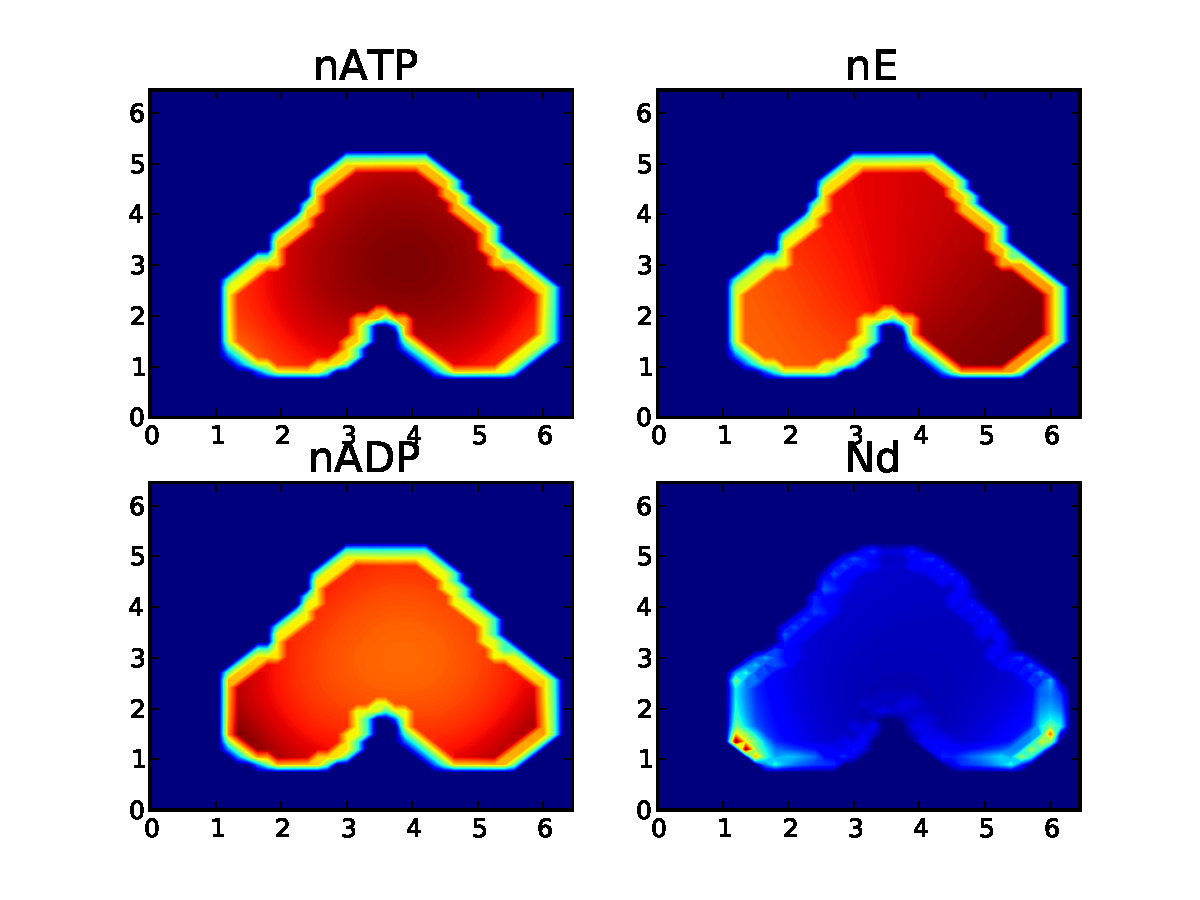
\includegraphics[width=\columnwidth]{../data/shape-randst/plots/time-map-compare-randst-10-60-60-990-150.pdf}
  \caption{randst 99}
  %\label{}
\end{figure}
\begin{figure}
  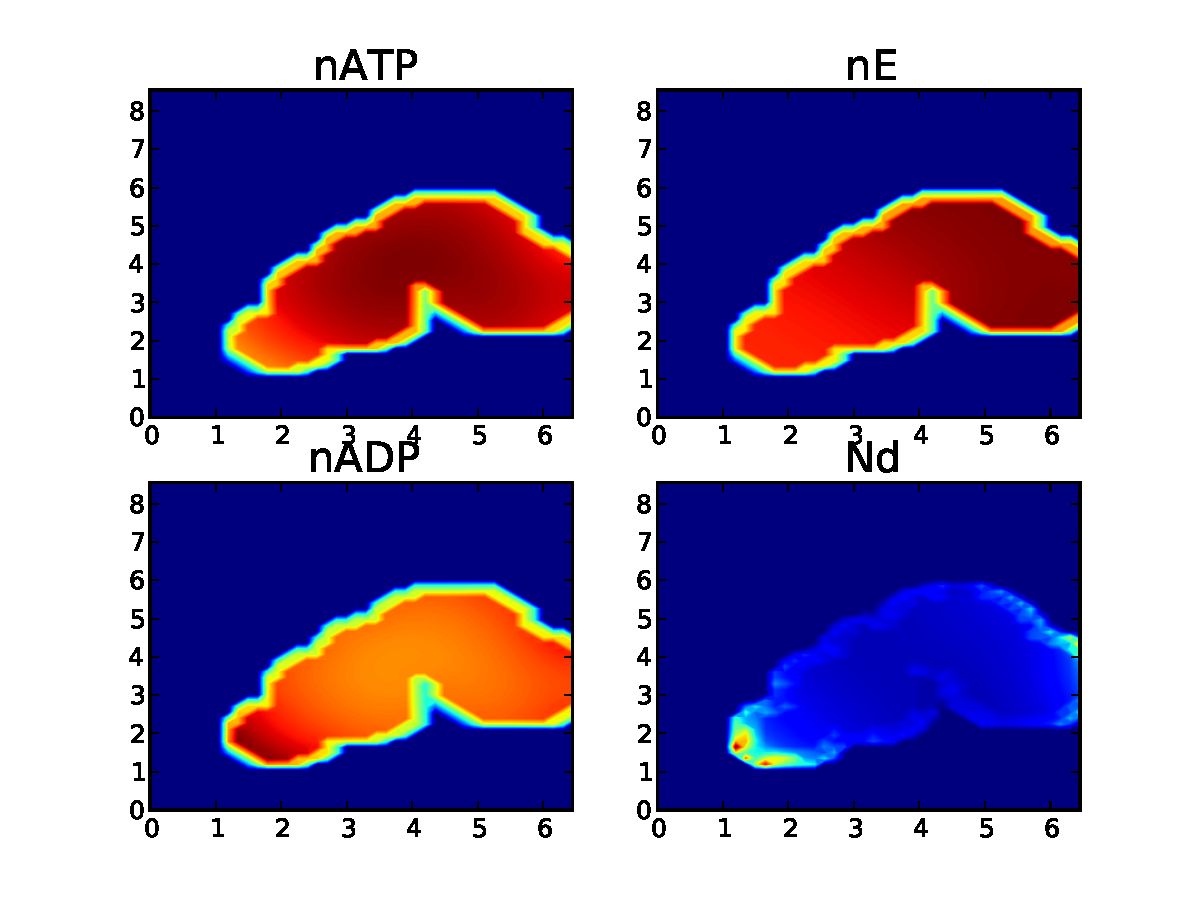
\includegraphics[width=\columnwidth]{../data/shape-randst/plots/time-map-compare-randst-10-80-60-980-150.pdf}
  \caption{randst 98}
  %\label{fig:pair-distribution-3}
\end{figure}
\begin{figure}
  \includegraphics[width=\columnwidth]{../data/shape-randst/plots/time-map-compare-randst-10-60-60-970-150.pdf}
  \caption{randst 97}
  %\label{fig:pair-distribution-3}
\end{figure}
\begin{figure}
  \includegraphics[width=\columnwidth]{../data/shape-randst/plots/time-map-compare-randst-10-60-60-960-150.pdf}
  \caption{randst 96}
  %\label{fig:pair-distribution-3}
\end{figure}

Randst 98 -

Randst 97 -

Randst 96 -

Triangle -


\section{Interpretation of Data}
-Discussion of conceptual reasons of why we see what we see
-Plots that are more interpretive (area-rating)
-Some sort of predictive claim?


\section{Conclusion}


\appendix

\section*{Appendix}


\end{document}
